\hypertarget{two-link-simulation}{%
\section{Two Link Simulation}\label{two-link-simulation}}

\hypertarget{position-computations}{%
\subsection{Position Computations}\label{position-computations}}

In this section we walk through some very simple computations seen in
the previous chapters. It also shows how we can use Julia as a
computational tool like seen with Matlab or Python. This chapter is not
intended to teach Julia. Julia is a modern programming language which is
well documented at \url{https://docs.julialang.org} . The language is
pretty easy to follow and if you have a background in any standard
procedural programming language, Julia is easy to read.

The Julia code to do the forward kinematics for the two link manipulator
is

\hypertarget{listFKTwoLink}{%
\label{listFKTwoLink}}%
\begin{Shaded}
\begin{Highlighting}[]
\NormalTok{a1}\OperatorTok{,}\NormalTok{a2 }\OperatorTok{=} \FloatTok{15.0}\OperatorTok{,}\FloatTok{10.0}
\NormalTok{t1}\OperatorTok{,}\NormalTok{ t2 }\OperatorTok{=} \FloatTok{0.1}\OperatorTok{,} \FloatTok{0.2}
\NormalTok{x }\OperatorTok{=}\NormalTok{ a2}\OperatorTok{*}\NormalTok{cos(t1}\OperatorTok{+}\NormalTok{t2) }\OperatorTok{+}\NormalTok{ a1}\OperatorTok{*}\NormalTok{cos(t1)}
\NormalTok{y }\OperatorTok{=}\NormalTok{ a2}\OperatorTok{*}\NormalTok{sin(t1}\OperatorTok{+}\NormalTok{t2) }\OperatorTok{+}\NormalTok{ a1}\OperatorTok{*}\NormalTok{sin(t1)}
\NormalTok{println(}\StringTok{"x = "}\OperatorTok{,}\NormalTok{ x}\OperatorTok{,} \StringTok{", y = "}\OperatorTok{,}\NormalTok{ y)}
\end{Highlighting}
\end{Shaded}

The Julia code to do the Inverse Kinematics for the Two Link Manipulator
follows. The computation is check by plugging the computed values into
the forward kinematics formula.

\hypertarget{listIKTwoLink}{%
\label{listIKTwoLink}}%
\begin{Shaded}
\begin{Highlighting}[]
\NormalTok{a1}\OperatorTok{,}\NormalTok{a2 }\OperatorTok{=} \FloatTok{15.0}\OperatorTok{,}\FloatTok{10.0}
\NormalTok{x}\OperatorTok{,}\NormalTok{y }\OperatorTok{=} \FloatTok{10.0}\OperatorTok{,}\FloatTok{8.0}
\NormalTok{d }\OperatorTok{=}\NormalTok{  (x}\OperatorTok{*}\NormalTok{x}\OperatorTok{+}\NormalTok{y}\OperatorTok{*}\NormalTok{y}\OperatorTok{{-}}\NormalTok{a1}\OperatorTok{*}\NormalTok{a1}\OperatorTok{{-}}\NormalTok{a2}\OperatorTok{*}\NormalTok{a2)}\OperatorTok{/}\NormalTok{(}\FloatTok{2}\OperatorTok{*}\NormalTok{a1}\OperatorTok{*}\NormalTok{a2)}
\NormalTok{println(}\StringTok{"x = "}\OperatorTok{,}\NormalTok{ x}\OperatorTok{,} \StringTok{" y = "}\OperatorTok{,}\NormalTok{ y)}
\NormalTok{println(}\StringTok{"d = "}\OperatorTok{,}\NormalTok{ d)}

\NormalTok{t2 }\OperatorTok{=}\NormalTok{ atan(}\OperatorTok{{-}}\NormalTok{sqrt(}\FloatTok{1.0}\OperatorTok{{-}}\NormalTok{d}\OperatorTok{*}\NormalTok{d)}\OperatorTok{,}\NormalTok{d)}
\NormalTok{t1 }\OperatorTok{=}\NormalTok{ atan(y}\OperatorTok{,}\NormalTok{x) }\OperatorTok{{-}}\NormalTok{ atan(a2}\OperatorTok{*}\NormalTok{sin(t2)}\OperatorTok{,}\NormalTok{a1}\OperatorTok{+}\NormalTok{a2}\OperatorTok{*}\NormalTok{cos(t2))}
\NormalTok{println(}\StringTok{"Angles:  t1 ="}\OperatorTok{,}\NormalTok{ t1}\OperatorTok{,}\StringTok{",  t2 = "}\OperatorTok{,}\NormalTok{ t2)}

\NormalTok{x1 }\OperatorTok{=}\NormalTok{ a2}\OperatorTok{*}\NormalTok{cos(t1}\OperatorTok{+}\NormalTok{t2) }\OperatorTok{+}\NormalTok{ a1}\OperatorTok{*}\NormalTok{cos(t1)}
\NormalTok{y1 }\OperatorTok{=}\NormalTok{ a2}\OperatorTok{*}\NormalTok{sin(t1}\OperatorTok{+}\NormalTok{t2) }\OperatorTok{+}\NormalTok{ a1}\OperatorTok{*}\NormalTok{sin(t1)}
\NormalTok{println(}\StringTok{"Check: x = "}\OperatorTok{,}\NormalTok{ x1}\OperatorTok{,} \StringTok{", y = "}\OperatorTok{,}\NormalTok{ y1)}
\end{Highlighting}
\end{Shaded}

The code to compute the position for the Parallel Two LInk manipulator
based on the parameters is

\hypertarget{lst:FKParallelTwoLink}{%
\label{lst:FKParallelTwoLink}}%
\begin{Shaded}
\begin{Highlighting}[]
\NormalTok{L0}\OperatorTok{,}\NormalTok{L1}\OperatorTok{,}\NormalTok{L2 }\OperatorTok{=} \FloatTok{8}\OperatorTok{,} \FloatTok{5}\OperatorTok{,} \FloatTok{10}
\NormalTok{th1 }\OperatorTok{=} \FloatTok{0.7}
\NormalTok{th2 }\OperatorTok{=} \FloatTok{0.8}

\NormalTok{a }\OperatorTok{=} \OperatorTok{{-}}\NormalTok{L1}\OperatorTok{*}\NormalTok{cos(th1)}\OperatorTok{{-}}\NormalTok{L0}\OperatorTok{/}\FloatTok{2.0}
\NormalTok{b }\OperatorTok{=}\NormalTok{ L1}\OperatorTok{*}\NormalTok{sin(th1)}
\NormalTok{c }\OperatorTok{=}\NormalTok{  L1}\OperatorTok{*}\NormalTok{cos(th2)}\OperatorTok{+}\NormalTok{L0}\OperatorTok{/}\FloatTok{2.0}
\NormalTok{d }\OperatorTok{=}\NormalTok{ L1}\OperatorTok{*}\NormalTok{sin(th2)}
\NormalTok{u }\OperatorTok{=}\NormalTok{ sqrt((a}\OperatorTok{{-}}\NormalTok{c)}\OperatorTok{\^{}}\FloatTok{2} \OperatorTok{+}\NormalTok{(b}\OperatorTok{{-}}\NormalTok{d)}\OperatorTok{\^{}}\FloatTok{2}\NormalTok{)}
\NormalTok{v }\OperatorTok{=}\NormalTok{ sqrt(L2}\OperatorTok{\^{}}\FloatTok{2} \OperatorTok{{-}}\NormalTok{ (u}\OperatorTok{\^{}}\FloatTok{2}\NormalTok{)}\OperatorTok{/}\FloatTok{4.0}\NormalTok{)}

\NormalTok{x }\OperatorTok{=}\NormalTok{ (a}\OperatorTok{+}\NormalTok{c)}\OperatorTok{/}\FloatTok{2.0} \OperatorTok{+}\NormalTok{ v}\OperatorTok{*}\NormalTok{(b}\OperatorTok{{-}}\NormalTok{d)}\OperatorTok{/}\NormalTok{u}
\NormalTok{y }\OperatorTok{=}\NormalTok{ (b}\OperatorTok{+}\NormalTok{d)}\OperatorTok{/}\FloatTok{2.0} \OperatorTok{+}\NormalTok{ v}\OperatorTok{*}\NormalTok{(c}\OperatorTok{{-}}\NormalTok{a)}\OperatorTok{/}\NormalTok{u}

\NormalTok{println(}\StringTok{"x = "}\OperatorTok{,}\NormalTok{ x}\OperatorTok{,}\StringTok{",  y = "}\OperatorTok{,}\NormalTok{y)}
\end{Highlighting}
\end{Shaded}

The inverse kinematics for the parallel two link manipulator is given by

\hypertarget{lst:IKParallelTwoLink}{%
\label{lst:IKParallelTwoLink}}%
\begin{Shaded}
\begin{Highlighting}[]
\NormalTok{L0}\OperatorTok{,}\NormalTok{L1}\OperatorTok{,}\NormalTok{L2 }\OperatorTok{=} \FloatTok{8}\OperatorTok{,} \FloatTok{5}\OperatorTok{,} \FloatTok{10}
\NormalTok{x}\OperatorTok{,}\NormalTok{ y }\OperatorTok{=} \OperatorTok{{-}}\FloatTok{0.5}\OperatorTok{,} \FloatTok{9}


\NormalTok{G }\OperatorTok{=}\NormalTok{ sqrt((x}\OperatorTok{{-}}\NormalTok{L0}\OperatorTok{/}\FloatTok{2.0}\NormalTok{)}\OperatorTok{*}\NormalTok{(x}\OperatorTok{{-}}\NormalTok{L0}\OperatorTok{/}\FloatTok{2.0}\NormalTok{)}\OperatorTok{+}\NormalTok{y}\OperatorTok{*}\NormalTok{y)}
\NormalTok{H }\OperatorTok{=}\NormalTok{ sqrt((x}\OperatorTok{+}\NormalTok{L0}\OperatorTok{/}\FloatTok{2.0}\NormalTok{)}\OperatorTok{*}\NormalTok{(x}\OperatorTok{+}\NormalTok{L0}\OperatorTok{/}\FloatTok{2.0}\NormalTok{)}\OperatorTok{+}\NormalTok{y}\OperatorTok{*}\NormalTok{y)}

\NormalTok{alpha }\OperatorTok{=}\NormalTok{ acos((G}\OperatorTok{*}\NormalTok{G }\OperatorTok{+}\NormalTok{ L0}\OperatorTok{*}\NormalTok{L0 }\OperatorTok{{-}}\NormalTok{ H}\OperatorTok{*}\NormalTok{H)}\OperatorTok{/}\NormalTok{(}\FloatTok{2.0}\OperatorTok{*}\NormalTok{G}\OperatorTok{*}\NormalTok{L0))}
\NormalTok{beta }\OperatorTok{=}\NormalTok{ acos((H}\OperatorTok{*}\NormalTok{H }\OperatorTok{+}\NormalTok{ L0}\OperatorTok{*}\NormalTok{L0 }\OperatorTok{{-}}\NormalTok{ G}\OperatorTok{*}\NormalTok{G)}\OperatorTok{/}\NormalTok{(}\FloatTok{2.0}\OperatorTok{*}\NormalTok{H}\OperatorTok{*}\NormalTok{L0))}
\NormalTok{gamma }\OperatorTok{=}\NormalTok{ acos((G}\OperatorTok{*}\NormalTok{G }\OperatorTok{+}\NormalTok{ L1}\OperatorTok{*}\NormalTok{L1 }\OperatorTok{{-}}\NormalTok{ L2}\OperatorTok{*}\NormalTok{L2)}\OperatorTok{/}\NormalTok{(}\FloatTok{2.0}\OperatorTok{*}\NormalTok{G}\OperatorTok{*}\NormalTok{L1))}
\NormalTok{eta }\OperatorTok{=}\NormalTok{ acos((H}\OperatorTok{*}\NormalTok{H }\OperatorTok{+}\NormalTok{ L1}\OperatorTok{*}\NormalTok{L1 }\OperatorTok{{-}}\NormalTok{ L2}\OperatorTok{*}\NormalTok{L2)}\OperatorTok{/}\NormalTok{(}\FloatTok{2.0}\OperatorTok{*}\NormalTok{H}\OperatorTok{*}\NormalTok{L1))}

\NormalTok{th1 }\OperatorTok{=} \ConstantTok{pi} \OperatorTok{{-}}\NormalTok{ beta }\OperatorTok{{-}}\NormalTok{ eta}
\NormalTok{th2 }\OperatorTok{=} \ConstantTok{pi} \OperatorTok{{-}}\NormalTok{ alpha }\OperatorTok{{-}}\NormalTok{ gamma}

\NormalTok{println(}\StringTok{"Angles theta1 = "}\OperatorTok{,}\NormalTok{ th1}\OperatorTok{,} \StringTok{",  theta2 = "}\OperatorTok{,}\NormalTok{ th2)}
\end{Highlighting}
\end{Shaded}

\hypertarget{velocity-computations}{%
\subsection{Velocity computations}\label{velocity-computations}}

In addition to forward and inverse position kinematics, one may need to
compute the forward and inverse velocity kinematics. Starting with
\(x(t), y(t)\)

\[\begin{aligned}
\begin{matrix}
x = a_2\cos (\theta_1+\theta_2) + a_1 \cos (\theta_1)\\
y = a_2 \sin (\theta_1 +\theta_2) + a_1\sin (\theta_1)
\end{matrix}
\end{aligned}\]

we compute the derivatives

\[\displaystyle \frac{dx}{dt} = -a_2\sin (\theta_1+\theta_2) \left( \frac{d\theta_1}{dt} + \frac{d\theta_2}{dt} \right)
-  a_1 \sin (\theta_1) \left( \frac{d\theta_1}{dt}  \right)
=  \left( -a_2\sin (\theta_1+\theta_2) -  a_1 \sin (\theta_1) \right) \left( \frac{d\theta_1}{dt}  \right)
 -a_2\sin (\theta_1+\theta_2) \left(\frac{d\theta_2}{dt} \right)\]\[\displaystyle  \frac{dy}{dt} = a_2 \cos (\theta_1 +\theta_2) \left( \frac{d\theta_1}{dt} + \frac{d\theta_2}{dt} \right)
+ a_1\cos (\theta_1)  \left( \frac{d\theta_1}{dt}  \right)
=  \left( a_2\cos (\theta_1+\theta_2) +  a_1 \cos (\theta_1) \right) \left( \frac{d\theta_1}{dt}  \right)
 + a_2\cos (\theta_1+\theta_2) \left(\frac{d\theta_2}{dt} \right)\]

As an example, given the two link manipulator with the length of the
first link \(a_1 = 10\) and the second link \(a_2 = 10\). If
\(\theta_1 = 45^\circ\), \(\theta_2 = 45^\circ\),
\(d\theta_1/dt = 5^\circ s^{-1}\), \(d\theta_2/dt = 10^\circ s^{-1}\)
find \(x\), \(y\), \(dx/dt\) and \(dy/dt\).

\hypertarget{lst:FKvelocitytwolink}{%
\label{lst:FKvelocitytwolink}}%
\begin{Shaded}
\begin{Highlighting}[]
\NormalTok{a1}\OperatorTok{,}\NormalTok{a2 }\OperatorTok{=} \FloatTok{10.0}\OperatorTok{,}\FloatTok{10.0}
\NormalTok{θ}\FloatTok{1}\OperatorTok{,}\NormalTok{ θ}\FloatTok{2} \OperatorTok{=} \FloatTok{45}\OperatorTok{*}\NormalTok{(π}\OperatorTok{/}\FloatTok{180}\NormalTok{)}\OperatorTok{,} \FloatTok{45}\OperatorTok{*}\NormalTok{(π}\OperatorTok{/}\FloatTok{180}\NormalTok{)}
\NormalTok{θ}\FloatTok{1}\NormalTok{dot}\OperatorTok{,}\NormalTok{ θ}\FloatTok{2}\NormalTok{dot }\OperatorTok{=} \FloatTok{5}\OperatorTok{*}\NormalTok{(π}\OperatorTok{/}\FloatTok{180}\NormalTok{)}\OperatorTok{,}\FloatTok{10}\OperatorTok{*}\NormalTok{(π}\OperatorTok{/}\FloatTok{180}\NormalTok{)}
\NormalTok{x }\OperatorTok{=}\NormalTok{ a2}\OperatorTok{*}\NormalTok{cos(θ}\FloatTok{1}\OperatorTok{+}\NormalTok{θ}\FloatTok{2}\NormalTok{) }\OperatorTok{+}\NormalTok{ a1}\OperatorTok{*}\NormalTok{cos(θ}\FloatTok{1}\NormalTok{)}
\NormalTok{y }\OperatorTok{=}\NormalTok{ a2}\OperatorTok{*}\NormalTok{sin(θ}\FloatTok{1}\OperatorTok{+}\NormalTok{θ}\FloatTok{2}\NormalTok{) }\OperatorTok{+}\NormalTok{ a1}\OperatorTok{*}\NormalTok{sin(θ}\FloatTok{1}\NormalTok{)}
\NormalTok{xdot }\OperatorTok{=} \OperatorTok{{-}}\NormalTok{(a2}\OperatorTok{*}\NormalTok{sin(θ}\FloatTok{1}\OperatorTok{+}\NormalTok{θ}\FloatTok{2}\NormalTok{) }\OperatorTok{+}\NormalTok{ a1}\OperatorTok{*}\NormalTok{sin(θ}\FloatTok{1}\NormalTok{))}\OperatorTok{*}\NormalTok{θ}\FloatTok{1}\NormalTok{dot }\OperatorTok{{-}}\NormalTok{ (a2}\OperatorTok{*}\NormalTok{sin(θ}\FloatTok{1}\OperatorTok{+}\NormalTok{θ}\FloatTok{2}\NormalTok{))}\OperatorTok{*}\NormalTok{θ}\FloatTok{2}\NormalTok{dot}
\NormalTok{ydot }\OperatorTok{=}\NormalTok{ (a2}\OperatorTok{*}\NormalTok{cos(θ}\FloatTok{1}\OperatorTok{+}\NormalTok{θ}\FloatTok{2}\NormalTok{) }\OperatorTok{+}\NormalTok{ a1}\OperatorTok{*}\NormalTok{cos(θ}\FloatTok{1}\NormalTok{))}\OperatorTok{*}\NormalTok{θ}\FloatTok{1}\NormalTok{dot }\OperatorTok{+}\NormalTok{  (a2}\OperatorTok{*}\NormalTok{cos(θ}\FloatTok{1}\OperatorTok{+}\NormalTok{θ}\FloatTok{2}\NormalTok{))}\OperatorTok{*}\NormalTok{θ}\FloatTok{2}\NormalTok{dot}
\NormalTok{println(}\StringTok{"x = "}\OperatorTok{,}\NormalTok{ x}\OperatorTok{,} \StringTok{", y = "}\OperatorTok{,}\NormalTok{ y}\OperatorTok{,} \StringTok{", xdot = "}\OperatorTok{,}\NormalTok{ xdot}\OperatorTok{,} \StringTok{", ydot = "}\OperatorTok{,}\NormalTok{ ydot)}
\end{Highlighting}
\end{Shaded}

Because the equations are linear in the rate variables, it is much
easier to to solve for the joint velocities as a function of linear
velocities. In this case, the matrix for the 2x2 system is

\[\begin{aligned}
A = \begin{bmatrix}
\left( -a_2\sin (\theta_1+\theta_2) -  a_1 \sin (\theta_1) \right) & -a_2\sin (\theta_1+\theta_2) \\
\left( a_2\cos (\theta_1+\theta_2) +  a_1 \cos (\theta_1) \right)  & a_2\cos (\theta_1+\theta_2)
\end{bmatrix}
\end{aligned}\]

where we have

\[\begin{aligned}
\begin{pmatrix} dx/dt\\  dy/dt \end{pmatrix} = A \begin{pmatrix} d\theta_1/dt \\ d\theta_2/dt \end{pmatrix}
\quad \Rightarrow \quad
\begin{pmatrix} d\theta_1/dt \\ d\theta_2/dt \end{pmatrix} = A^{-1} \begin{pmatrix} dx/dt\\  dy/dt \end{pmatrix}
\end{aligned}\]

The inverse of the matrix is

\[\begin{aligned}
A^{-1} = \frac{1}{a_1a_2\sin(\theta_2)}
\begin{bmatrix}
 a_2\cos (\theta_1+\theta_2) & a_2\sin (\theta_1+\theta_2) \\
- \left( a_2\cos (\theta_1+\theta_2) +  a_1 \cos (\theta_1) \right)  &
-\left(a_2\sin (\theta_1+\theta_2) +  a_1 \sin (\theta_1) \right)
\end{bmatrix}
\end{aligned}\]

This gives use the velocity formulas for the inverse kinematics:

\[\frac{d\theta_1}{dt} = \frac{1}{a_1a_2\sin(\theta_2)} \left[  a_2\cos (\theta_1+\theta_2) \frac{dx}{dt}
+ a_2\sin (\theta_1+\theta_2) \frac{dy}{dt} \right]\]\[\frac{d\theta_2}{dt} = - \frac{1}{a_1a_2\sin(\theta_2)} \left[  \left( a_2\cos (\theta_1+\theta_2) +  a_1 \cos (\theta_1) \right)  \frac{dx}{dt} +
\left(a_2\sin (\theta_1+\theta_2) +  a_1 \sin (\theta_1) \right) \frac{dy}{dt} \right]\]

We can gain \(\theta_1, \theta_2\) from the inverse kinematics formulas.

Example Given the two link manipulator as above with the length of the
first link \(a_1 = 10\) and the second link \(a_2 = 10\). If \(x = 12\),
\(y = 14\), \(dx/dt = -0.25\), \(dy/dt = 0.5\), find \(d\theta_1/dt\)
and \(d\theta_2/dt\)

\hypertarget{lst:IKvelocitytwolink}{%
\label{lst:IKvelocitytwolink}}%
\begin{Shaded}
\begin{Highlighting}[]
\NormalTok{a1}\OperatorTok{,}\NormalTok{a2 }\OperatorTok{=} \FloatTok{10.0}\OperatorTok{,}\FloatTok{10.0}
\NormalTok{x}\OperatorTok{,}\NormalTok{y }\OperatorTok{=} \FloatTok{12}\OperatorTok{,} \FloatTok{14}
\NormalTok{xdot}\OperatorTok{,}\NormalTok{ ydot }\OperatorTok{=} \OperatorTok{{-}}\FloatTok{0.25}\OperatorTok{,} \FloatTok{0.5}
\NormalTok{d }\OperatorTok{=}\NormalTok{  (x}\OperatorTok{*}\NormalTok{x}\OperatorTok{+}\NormalTok{y}\OperatorTok{*}\NormalTok{y}\OperatorTok{{-}}\NormalTok{a1}\OperatorTok{*}\NormalTok{a1}\OperatorTok{{-}}\NormalTok{a2}\OperatorTok{*}\NormalTok{a2)}\OperatorTok{/}\NormalTok{(}\FloatTok{2}\OperatorTok{*}\NormalTok{a1}\OperatorTok{*}\NormalTok{a2)}
\NormalTok{θ}\FloatTok{2} \OperatorTok{=}\NormalTok{ atan(sqrt(}\FloatTok{1.0}\OperatorTok{{-}}\NormalTok{d}\OperatorTok{*}\NormalTok{d)}\OperatorTok{,}\NormalTok{d)}
\NormalTok{θ}\FloatTok{1} \OperatorTok{=}\NormalTok{ atan(y}\OperatorTok{,}\NormalTok{x) }\OperatorTok{{-}}\NormalTok{ atan(a2}\OperatorTok{*}\NormalTok{sin(θ}\FloatTok{2}\NormalTok{)}\OperatorTok{,}\NormalTok{a1}\OperatorTok{+}\NormalTok{a2}\OperatorTok{*}\NormalTok{cos(θ}\FloatTok{2}\NormalTok{))}
\NormalTok{r }\OperatorTok{=} \FloatTok{1.0}\OperatorTok{/}\NormalTok{(a1}\OperatorTok{*}\NormalTok{a2}\OperatorTok{*}\NormalTok{sin(θ}\FloatTok{2}\NormalTok{))}
\NormalTok{θ}\FloatTok{1}\NormalTok{dot }\OperatorTok{=}\NormalTok{ r}\OperatorTok{*}\NormalTok{(a2}\OperatorTok{*}\NormalTok{cos(θ}\FloatTok{1}\OperatorTok{+}\NormalTok{θ}\FloatTok{2}\NormalTok{)}\OperatorTok{*}\NormalTok{xdot }\OperatorTok{+}\NormalTok{ a2}\OperatorTok{*}\NormalTok{sin(θ}\FloatTok{1}\OperatorTok{+}\NormalTok{θ}\FloatTok{2}\NormalTok{)}\OperatorTok{*}\NormalTok{ydot)}
\NormalTok{θ}\FloatTok{2}\NormalTok{dot }\OperatorTok{=} \OperatorTok{{-}}\NormalTok{r}\OperatorTok{*}\NormalTok{(x}\OperatorTok{*}\NormalTok{xdot }\OperatorTok{+}\NormalTok{ y}\OperatorTok{*}\NormalTok{ydot)}
\NormalTok{println(}\StringTok{"θ1 = "}\OperatorTok{,} \FloatTok{180}\OperatorTok{*}\NormalTok{θ}\FloatTok{1}\OperatorTok{/}\NormalTok{π}\OperatorTok{,} \StringTok{", θ2 = "}\OperatorTok{,} \FloatTok{180}\OperatorTok{*}\NormalTok{θ}\FloatTok{2}\OperatorTok{/}\NormalTok{π}\OperatorTok{,} \StringTok{", θ1dot = "}\OperatorTok{,} \FloatTok{180}\OperatorTok{*}\NormalTok{θ}\FloatTok{1}\NormalTok{dot}\OperatorTok{/}\NormalTok{π}\OperatorTok{,} \StringTok{", θ2dot = "}\OperatorTok{,} \FloatTok{180}\OperatorTok{*}\NormalTok{θ}\FloatTok{2}\NormalTok{dot}\OperatorTok{/}\NormalTok{π)}
\end{Highlighting}
\end{Shaded}

\hypertarget{arm-computations}{%
\subsection{Arm computations}\label{arm-computations}}

In application we will want the robot end effector trace out a curve in
the workspace. A simple version of this would be to provide a sequence
of points for the arm to trace out. There are two curves that we have in
mind. One is the curve in the physical workspace and the other is the
corresponding curve in the parameter or Configuration space.

To drive a physical arm we send commands to the joints. This means we
are controlling the arm by driving it along a curve in configuration
space. A simple way to approach this is to create a sequence of points
in configuration space and then move the arm in short updates on the
joint angles. We will see in the next section a much smoother way to
approach this task however for now, this approach will get the
manipulator moving along the desired path.

\begin{figure}
\centering
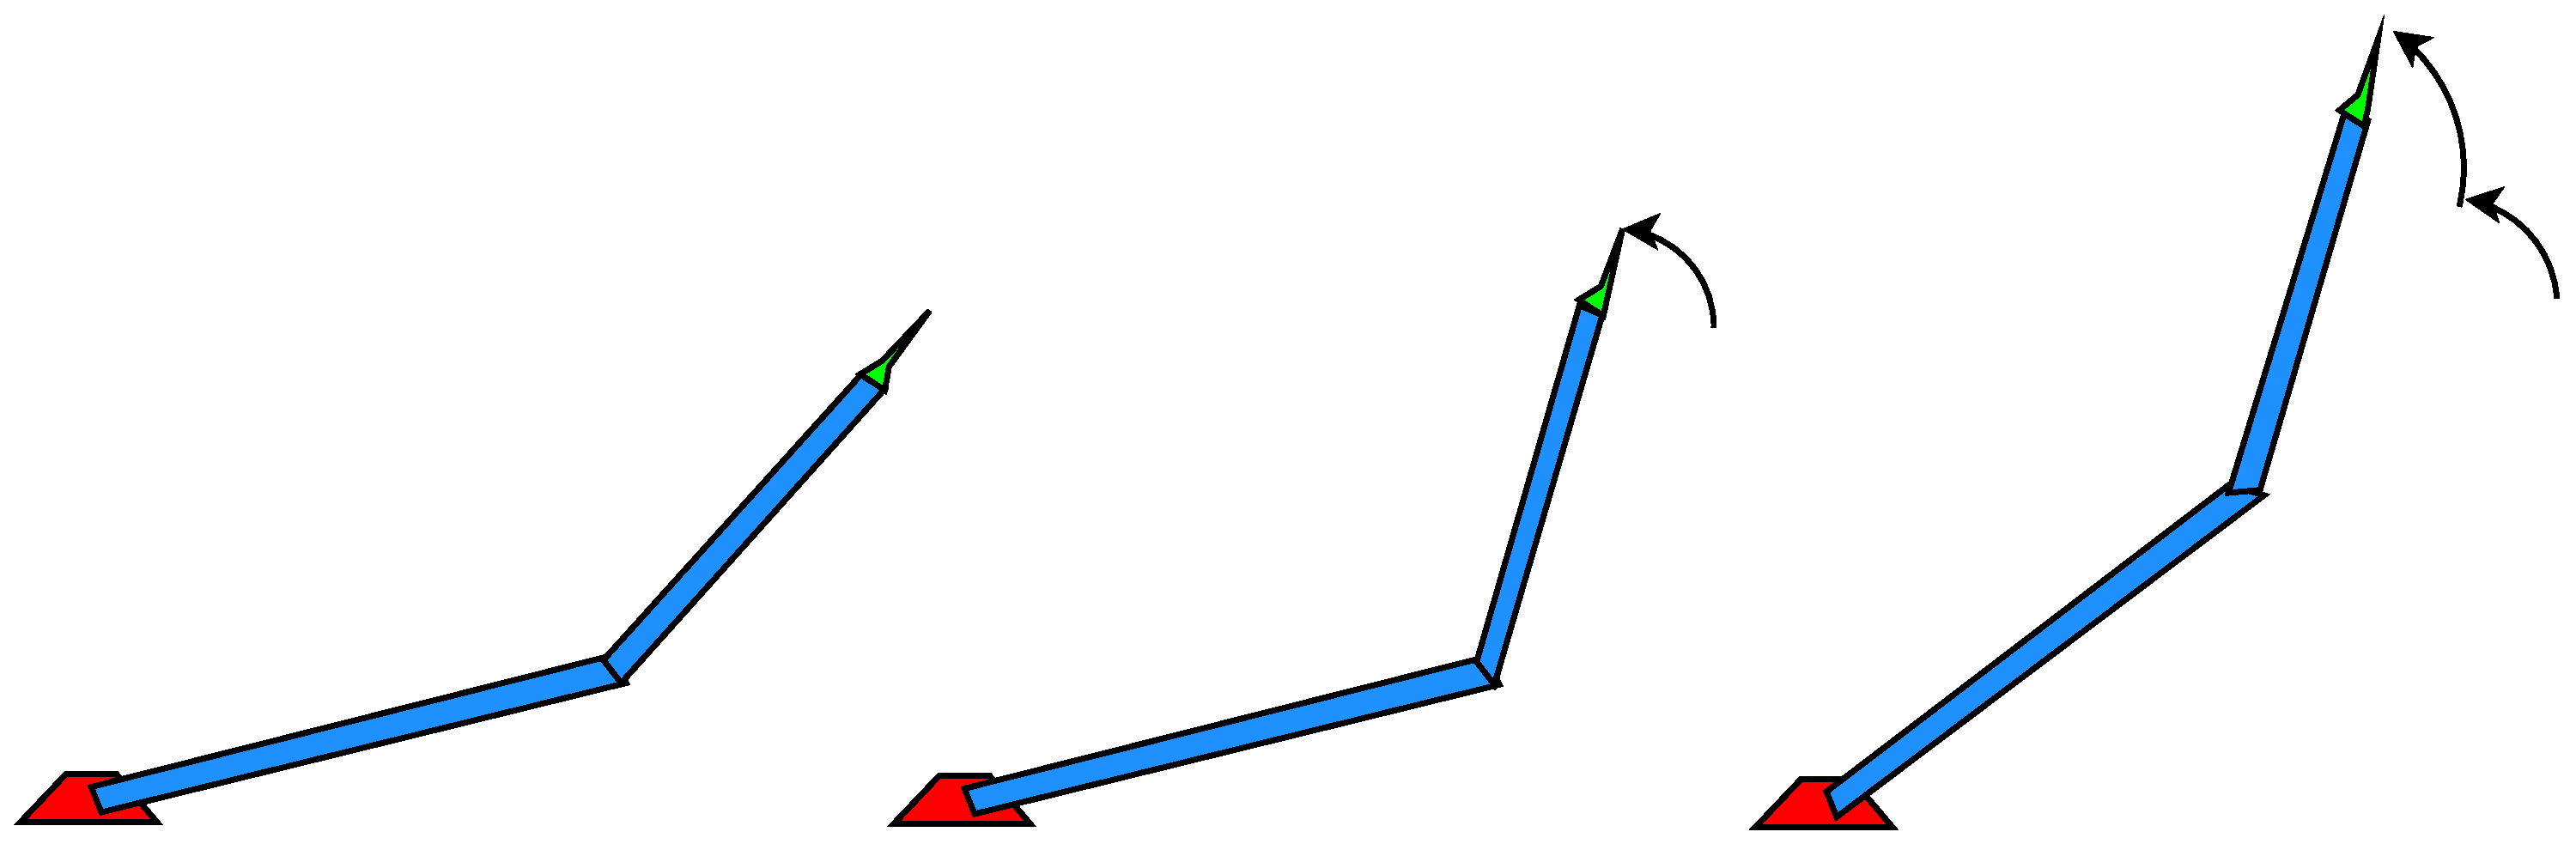
\includegraphics[width=0.5\textwidth,height=\textheight]{SimulationFigures/twolinkpositioncntrl.*}
\caption{Try a simple position control. Send a discrete set of control
points.}
\end{figure}

The workflow will be to parametrize the path in the workspace, then find
the curve in the parameter space using the inverse kinematics. To keep
things simple, we will assume the curve lies inside the reachable
workspace. The goal is then to have the arm trace out \(x(t)\) and
\(y(t)\). If we want to trace out

\[x(t) = t+1, \quad y(t) = 2t - 1\]

Where \(t\) ranges from 0 to 5 with 100 points. A simple Julia program
can generate the \((x,y)\) pairs:

\hypertarget{lst:mostbasicloop}{%
\label{lst:mostbasicloop}}%
\begin{Shaded}
\begin{Highlighting}[]
\KeywordTok{for}\NormalTok{ i }\OperatorTok{=} \FloatTok{1}\OperatorTok{:}\FloatTok{100}
\NormalTok{   t }\OperatorTok{=}\NormalTok{ i}\OperatorTok{/}\FloatTok{20}
\NormalTok{   x }\OperatorTok{=}\NormalTok{ t}\OperatorTok{+}\FloatTok{1}
\NormalTok{   y }\OperatorTok{=} \FloatTok{2}\OperatorTok{*}\NormalTok{t}\OperatorTok{{-}}\FloatTok{1}
\NormalTok{   println(}\StringTok{"("}\OperatorTok{,}\NormalTok{ x}\OperatorTok{,} \StringTok{", "}\OperatorTok{,}\NormalTok{y}\OperatorTok{,}\StringTok{")"}\NormalTok{)}
\KeywordTok{end}
\end{Highlighting}
\end{Shaded}

For most of our examples we will need to store the points in an array.
Julia has many ways to perform this and we will show a couple of
approaches.

\hypertarget{lst:basicloop}{%
\label{lst:basicloop}}%
\begin{Shaded}
\begin{Highlighting}[]
\NormalTok{N }\OperatorTok{=} \FloatTok{100}
\NormalTok{x }\OperatorTok{=}\NormalTok{ zeros(N)}
\NormalTok{y }\OperatorTok{=}\NormalTok{ zeros(N)}
\NormalTok{delta }\OperatorTok{=} \FloatTok{5}\OperatorTok{/}\NormalTok{N}

\KeywordTok{for}\NormalTok{ i }\OperatorTok{=} \FloatTok{1}\OperatorTok{:}\NormalTok{N}
\NormalTok{   t }\OperatorTok{=}\NormalTok{ delta}\OperatorTok{*}\NormalTok{i}
\NormalTok{   x[i]}\OperatorTok{=}\NormalTok{ t}\OperatorTok{+}\FloatTok{1}
\NormalTok{   y[i] }\OperatorTok{=} \FloatTok{2}\OperatorTok{*}\NormalTok{t}\OperatorTok{{-}}\FloatTok{1}
\KeywordTok{end}
\end{Highlighting}
\end{Shaded}

Julia supports implicit parallel computations in the same way found in
Python's Numpy. Using the LinRange constructor we can produce t
directly. Then x and y can be found by the elementwise dot operator.
Note the period in front of the binary operator.

\hypertarget{lst:basicimplicitloop}{%
\label{lst:basicimplicitloop}}%
\begin{Shaded}
\begin{Highlighting}[]
\NormalTok{t }\OperatorTok{=} \DataTypeTok{LinRange}\NormalTok{(}\FloatTok{0}\OperatorTok{,} \FloatTok{5}\OperatorTok{,} \FloatTok{100}\NormalTok{)}
\NormalTok{x }\OperatorTok{=}\NormalTok{  t .}\OperatorTok{+} \FloatTok{1.0}
\NormalTok{y }\OperatorTok{=} \FloatTok{2} \OperatorTok{.*}\NormalTok{ t .}\OperatorTok{{-}} \FloatTok{1.0}
\end{Highlighting}
\end{Shaded}

We can gain a plot of this easily by adding a couple of statements

\hypertarget{lst:basicplot}{%
\label{lst:basicplot}}%
\begin{Shaded}
\begin{Highlighting}[]
\KeywordTok{using}\NormalTok{ Plots}
\NormalTok{t }\OperatorTok{=} \DataTypeTok{LinRange}\NormalTok{(}\FloatTok{0}\OperatorTok{,} \FloatTok{5}\OperatorTok{,} \FloatTok{100}\NormalTok{)}
\NormalTok{x }\OperatorTok{=}\NormalTok{  t .}\OperatorTok{+} \FloatTok{1.0}
\NormalTok{y }\OperatorTok{=} \FloatTok{2} \OperatorTok{.*}\NormalTok{ t .}\OperatorTok{{-}} \FloatTok{1.0}
\NormalTok{display(plot(x}\OperatorTok{,}\NormalTok{y))}
\CommentTok{\#readline()}
\end{Highlighting}
\end{Shaded}

The readline() function is there to prevent the process from exiting
before the plot appears when you are using the REPL. This is not an
issue when using Jupyter and you can skip it. You also don't need the
display function wrapping the plot function when working in a Jupyter
notebook. Note - if you want to keep these plots, use the savefig
function: \emph{savefig("foo.svg")}. It will save the recent plot using
the extension as the file format. Figure \texttt{Fig:sampleline} is what
gets generated.

\begin{quote}
Sample plot generated by the plot function.
\end{quote}

You may have noticed that it took much longer than expected to get the
plot window (if you are used to Matlab or Python). Even though the
programs look very similar to Python, Julia is compiled (at run time).
The delay you experience is due to the compilation of the Plots package.
After the compile is completed, the program runs close to the speed of
C. For short programs you notice the delay due to the compile process.
So for the shorter scripts, it reduces the overall speed since each time
you run the script from the command line you recompile. If you plan to
run little experiments or plots, it is better to stay in the REPL (the
Julia interpreter) or a Jupyter Notebook since you only see the package
compile delay once per session.

For larger progams or longer running processes, the increase in speed
can be dramatic. This book will present the code as blocks that can be
copied to a file which allows one to run the file from the command line.
However, you may choose to cut and paste the code into the REPL or
Jupyter for faster plots so you are not recompiling on each script.
There is some variation is the plotting code to give some additional
examples.

We can enter the array of workspace points into the inverse kinematics
formulas. Then to check we take those points into the forward
kinematics. Plots for the configuration (parameter) space curve and then
the final workspace curve are produced.

\hypertarget{lst:basicfkandik}{%
\label{lst:basicfkandik}}%
\begin{Shaded}
\begin{Highlighting}[]
\KeywordTok{using}\NormalTok{ Plots}

\NormalTok{t }\OperatorTok{=} \DataTypeTok{LinRange}\NormalTok{(}\FloatTok{1}\OperatorTok{,} \FloatTok{5}\OperatorTok{,} \FloatTok{100}\NormalTok{)}
\NormalTok{x }\OperatorTok{=}\NormalTok{  t .}\OperatorTok{+} \FloatTok{1.0}
\NormalTok{y }\OperatorTok{=} \FloatTok{2} \OperatorTok{.*}\NormalTok{ t .}\OperatorTok{{-}} \FloatTok{1.0}
\NormalTok{a1}\OperatorTok{,}\NormalTok{a2 }\OperatorTok{=} \FloatTok{15.0}\OperatorTok{,}\FloatTok{15.0}
\NormalTok{d }\OperatorTok{=}\NormalTok{  ((x}\OperatorTok{.*}\NormalTok{x) .}\OperatorTok{+}\NormalTok{ (y}\OperatorTok{.*}\NormalTok{y) .}\OperatorTok{{-}}\NormalTok{ (a1}\OperatorTok{.*}\NormalTok{a1) .}\OperatorTok{{-}}\NormalTok{ (a2}\OperatorTok{.*}\NormalTok{a2))}\OperatorTok{/}\NormalTok{(}\FloatTok{2.0} \OperatorTok{.*}\NormalTok{ (a1}\OperatorTok{.*}\NormalTok{a2))}
\NormalTok{t2 }\OperatorTok{=}\NormalTok{ atan.(}\OperatorTok{{-}}\NormalTok{sqrt.(}\FloatTok{1.0}\NormalTok{ .}\OperatorTok{{-}}\NormalTok{ (d}\OperatorTok{.*}\NormalTok{d))}\OperatorTok{,}\NormalTok{d)}
\NormalTok{t1 }\OperatorTok{=}\NormalTok{ atan.(y}\OperatorTok{,}\NormalTok{x) }\OperatorTok{{-}}\NormalTok{ atan.(a2}\OperatorTok{.*}\NormalTok{sin.(t2)}\OperatorTok{,}\NormalTok{ a1 .}\OperatorTok{+}\NormalTok{ a2}\OperatorTok{.*}\NormalTok{cos.(t2))}

\NormalTok{display(plot(t1}\OperatorTok{,}\NormalTok{t2))}
\CommentTok{\#savefig("IK.svg")}
\CommentTok{\#readline()}
\NormalTok{x1 }\OperatorTok{=}\NormalTok{ a2}\OperatorTok{.*}\NormalTok{cos.(t1.}\OperatorTok{+}\NormalTok{t2) .}\OperatorTok{+}\NormalTok{ a1}\OperatorTok{.*}\NormalTok{cos.(t1)}
\NormalTok{y1 }\OperatorTok{=}\NormalTok{ a2}\OperatorTok{.*}\NormalTok{sin.(t1.}\OperatorTok{+}\NormalTok{t2) .}\OperatorTok{+}\NormalTok{ a1}\OperatorTok{.*}\NormalTok{sin.(t1)}
\NormalTok{display(plot(x1}\OperatorTok{,}\NormalTok{y1))}
\CommentTok{\#savefig("FK.svg")}
\CommentTok{\#readline()}







\NormalTok{First plot generated by }\OperatorTok{:}\NormalTok{numref}\OperatorTok{:}\SpecialStringTok{\textasciigrave{}lst:basicfkandik\textasciigrave{}}\NormalTok{ .}








\NormalTok{The check on the IK values from }\OperatorTok{:}\NormalTok{numref}\OperatorTok{:}\SpecialStringTok{\textasciigrave{}lst:basicfkandik\textasciigrave{}}\NormalTok{ .}
\end{Highlighting}
\end{Shaded}

For another two link example, determine the joint angles to trace out a
circle centered at (10,8) of radius 5 with \(a_1 = a_2 = 15\). The
circle can be parametrized by \(x(t) = 5\cos (t) + 10\),
\(y(t) = 5 \sin(t) + 8\), \(0 \leq t \leq 2\pi\). Generate an array of
points on the circle and plug them into the inverse kinematics. Julia
has a macro available \texttt{@.} that can replace the binary operators
with their dotted operators. It is very handy in translating to a vector
formulation.

\hypertarget{lst:circletrace}{%
\label{lst:circletrace}}%
\begin{Shaded}
\begin{Highlighting}[]
\KeywordTok{using}\NormalTok{ Plots}

\NormalTok{t }\OperatorTok{=} \DataTypeTok{LinRange}\NormalTok{(}\FloatTok{0}\OperatorTok{,} \FloatTok{6.28318530718}\OperatorTok{,} \FloatTok{100}\NormalTok{)}
\NormalTok{x }\OperatorTok{=} \OperatorTok{@}\NormalTok{. }\FloatTok{5} \OperatorTok{*}\NormalTok{ cos(t) }\OperatorTok{+} \FloatTok{10.0}
\NormalTok{y }\OperatorTok{=} \OperatorTok{@}\NormalTok{. }\FloatTok{5} \OperatorTok{*}\NormalTok{ sin(t) }\OperatorTok{+} \FloatTok{8.0}
\NormalTok{a1}\OperatorTok{,}\NormalTok{a2 }\OperatorTok{=} \FloatTok{15.0}\OperatorTok{,}\FloatTok{15.0}
\NormalTok{d }\OperatorTok{=}  \OperatorTok{@}\NormalTok{. ((x}\OperatorTok{*}\NormalTok{x) }\OperatorTok{+}\NormalTok{ (y}\OperatorTok{*}\NormalTok{y) }\OperatorTok{{-}}\NormalTok{ (a1}\OperatorTok{*}\NormalTok{a1) }\OperatorTok{{-}}\NormalTok{ (a2}\OperatorTok{*}\NormalTok{a2))}\OperatorTok{/}\NormalTok{(}\FloatTok{2.0} \OperatorTok{*}\NormalTok{ (a1}\OperatorTok{*}\NormalTok{a2))}
\NormalTok{t2 }\OperatorTok{=} \OperatorTok{@}\NormalTok{. atan(}\OperatorTok{{-}}\NormalTok{sqrt(}\FloatTok{1.0} \OperatorTok{{-}}\NormalTok{ (d}\OperatorTok{*}\NormalTok{d))}\OperatorTok{,}\NormalTok{d)}
\NormalTok{t1 }\OperatorTok{=} \OperatorTok{@}\NormalTok{. atan(y}\OperatorTok{,}\NormalTok{x) }\OperatorTok{{-}}\NormalTok{ atan(a2}\OperatorTok{*}\NormalTok{sin(t2)}\OperatorTok{,}\NormalTok{ a1 }\OperatorTok{+}\NormalTok{ a2}\OperatorTok{*}\NormalTok{cos(t2))}

\NormalTok{display(plot(t1}\OperatorTok{,}\NormalTok{t2))}
\NormalTok{savefig(}\StringTok{"IK.svg"}\NormalTok{)}
\CommentTok{\#readline()}
\NormalTok{x1 }\OperatorTok{=} \OperatorTok{@}\NormalTok{. a2}\OperatorTok{*}\NormalTok{cos(t1}\OperatorTok{+}\NormalTok{t2) }\OperatorTok{+}\NormalTok{ a1}\OperatorTok{*}\NormalTok{cos(t1)}
\NormalTok{y1 }\OperatorTok{=} \OperatorTok{@}\NormalTok{. a2}\OperatorTok{*}\NormalTok{sin(t1}\OperatorTok{+}\NormalTok{t2) }\OperatorTok{+}\NormalTok{ a1}\OperatorTok{*}\NormalTok{sin(t1)}
\NormalTok{display(plot(x1}\OperatorTok{,}\NormalTok{y1))}
\NormalTok{savefig(}\StringTok{"FK.svg"}\NormalTok{)}
\CommentTok{\#readline()}









\NormalTok{Plot generated by }\OperatorTok{:}\NormalTok{numref}\OperatorTok{:}\SpecialStringTok{\textasciigrave{}lst:circletrace\textasciigrave{}}\NormalTok{ .}
\end{Highlighting}
\end{Shaded}

The implicit formulation above is very similar to how one might approach
developing code for Numpy. The traditional approach works well and does
not require that much additional code. You can see the loops explicitly
which is not always a bad thing.

\hypertarget{listIKTwoLinkFunction}{%
\label{listIKTwoLinkFunction}}%
\begin{Shaded}
\begin{Highlighting}[]
\KeywordTok{function}\NormalTok{ ik(x}\OperatorTok{,}\NormalTok{ y}\OperatorTok{,}\NormalTok{ a1}\OperatorTok{,}\NormalTok{ a2)}
\NormalTok{   d }\OperatorTok{=}\NormalTok{  (x}\OperatorTok{*}\NormalTok{x}\OperatorTok{+}\NormalTok{y}\OperatorTok{*}\NormalTok{y}\OperatorTok{{-}}\NormalTok{a1}\OperatorTok{*}\NormalTok{a1}\OperatorTok{{-}}\NormalTok{a2}\OperatorTok{*}\NormalTok{a2)}\OperatorTok{/}\NormalTok{(}\FloatTok{2}\OperatorTok{*}\NormalTok{a1}\OperatorTok{*}\NormalTok{a2)}
\NormalTok{   th2 }\OperatorTok{=}\NormalTok{ atan(}\OperatorTok{{-}}\NormalTok{sqrt(}\FloatTok{1.0}\OperatorTok{{-}}\NormalTok{d}\OperatorTok{*}\NormalTok{d)}\OperatorTok{,}\NormalTok{d)}
\NormalTok{   th1 }\OperatorTok{=}\NormalTok{ atan(y}\OperatorTok{,}\NormalTok{x) }\OperatorTok{{-}}\NormalTok{ atan(a2}\OperatorTok{*}\NormalTok{sin(th2)}\OperatorTok{,}\NormalTok{a1}\OperatorTok{+}\NormalTok{a2}\OperatorTok{*}\NormalTok{cos(th2))}
   \KeywordTok{return}\NormalTok{ (th1}\OperatorTok{,}\NormalTok{th2)}
\KeywordTok{end}


\KeywordTok{function}\NormalTok{ fk(t1}\OperatorTok{,}\NormalTok{ t2}\OperatorTok{,}\NormalTok{ a1}\OperatorTok{,}\NormalTok{ a2)}
\NormalTok{    x }\OperatorTok{=}\NormalTok{ a2}\OperatorTok{*}\NormalTok{cos(t1}\OperatorTok{+}\NormalTok{t2) }\OperatorTok{+}\NormalTok{ a1}\OperatorTok{*}\NormalTok{cos(t1)}
\NormalTok{    y }\OperatorTok{=}\NormalTok{ a2}\OperatorTok{*}\NormalTok{sin(t1}\OperatorTok{+}\NormalTok{t2) }\OperatorTok{+}\NormalTok{ a1}\OperatorTok{*}\NormalTok{sin(t1)}
    \KeywordTok{return}\NormalTok{ x}\OperatorTok{,}\NormalTok{y}
\KeywordTok{end}

\NormalTok{a1}\OperatorTok{,}\NormalTok{ a2 }\OperatorTok{=} \FloatTok{15.0}\OperatorTok{,} \FloatTok{15.0}

\NormalTok{t1 }\OperatorTok{=}\NormalTok{ zeros(}\FloatTok{10}\NormalTok{)}
\NormalTok{t2 }\OperatorTok{=}\NormalTok{ zeros(}\FloatTok{10}\NormalTok{)}

\KeywordTok{for}\NormalTok{ i }\OperatorTok{=} \FloatTok{1}\OperatorTok{:}\FloatTok{10}
    \KeywordTok{global}\NormalTok{ a1}\OperatorTok{,}\NormalTok{ a2}\OperatorTok{,}\NormalTok{ t1}\OperatorTok{,}\NormalTok{ t2}
\NormalTok{    x }\OperatorTok{=} \FloatTok{9} \OperatorTok{+} \FloatTok{0.1}\OperatorTok{*}\NormalTok{i}
\NormalTok{    y }\OperatorTok{=} \FloatTok{7} \OperatorTok{+} \FloatTok{0.1}\OperatorTok{*}\NormalTok{i}
\NormalTok{   (t1[i]}\OperatorTok{,}\NormalTok{ t2[i]) }\OperatorTok{=}\NormalTok{ ik(x}\OperatorTok{,}\NormalTok{ y}\OperatorTok{,}\NormalTok{ a1}\OperatorTok{,}\NormalTok{ a2)}
\NormalTok{   x1}\OperatorTok{,}\NormalTok{ y1 }\OperatorTok{=}\NormalTok{ fk(t1[i]}\OperatorTok{,}\NormalTok{ t2[i]}\OperatorTok{,}\NormalTok{ a1}\OperatorTok{,}\NormalTok{ a2)}
\NormalTok{   println((x}\OperatorTok{{-}}\NormalTok{x1)}\OperatorTok{\^{}}\FloatTok{2} \OperatorTok{+}\NormalTok{ (y}\OperatorTok{{-}}\NormalTok{y1)}\OperatorTok{*}\FloatTok{2}\NormalTok{)}
\KeywordTok{end}
\NormalTok{p}\OperatorTok{=}\NormalTok{plot(t1}\OperatorTok{,}\NormalTok{t2)}
\NormalTok{display(p)}
\CommentTok{\#readline()}
\end{Highlighting}
\end{Shaded}

\hypertarget{parallel-two-link-computations}{%
\subsection{Parallel Two Link
Computations}\label{parallel-two-link-computations}}

The following sbows the code used to produce the parallel manipulator
workspace shown in \texttt{Fig:paralleltwolinkWS} . uses a double loop
over \(\theta_1\) and \(\theta_2\), which places these values in the
forward kinematics and then gathers the resulting \((x,y)\) values. Like
the serial manipulator, this is a holonomic robot as well.

\hypertarget{lst:computeconfigdomain}{%
\label{lst:computeconfigdomain}}%
\begin{Shaded}
\begin{Highlighting}[]
\KeywordTok{using}\NormalTok{ Plots}

\CommentTok{\# Set the link lengths}
\NormalTok{L0 }\OperatorTok{=} \FloatTok{8}
\NormalTok{L1 }\OperatorTok{=} \FloatTok{5}
\NormalTok{L2 }\OperatorTok{=} \FloatTok{10}

\CommentTok{\# Initialize the arrays}
\NormalTok{xlist }\OperatorTok{=}\NormalTok{ zeros(}\FloatTok{0}\NormalTok{)}
\NormalTok{ylist }\OperatorTok{=}\NormalTok{ zeros(}\FloatTok{0}\NormalTok{)}

\CommentTok{\# Loop over the two angles,}
\CommentTok{\#  stepping about 1.8 degrees each step}

\KeywordTok{for}\NormalTok{ i }\OperatorTok{=} \FloatTok{1}\OperatorTok{:}\FloatTok{100}
   \KeywordTok{for}\NormalTok{ j }\OperatorTok{=} \FloatTok{1}\OperatorTok{:}\FloatTok{100}
\NormalTok{      th1 }\OperatorTok{=} \FloatTok{0} \OperatorTok{+} \FloatTok{1.57}\OperatorTok{*}\NormalTok{i}\OperatorTok{/}\FloatTok{100.0}
\NormalTok{      th2 }\OperatorTok{=} \FloatTok{0} \OperatorTok{+} \FloatTok{1.57}\OperatorTok{*}\NormalTok{j}\OperatorTok{/}\FloatTok{100.0}

\NormalTok{      a }\OperatorTok{=} \OperatorTok{{-}}\NormalTok{L1}\OperatorTok{*}\NormalTok{cos(th1) }\OperatorTok{{-}}\NormalTok{ L0}\OperatorTok{/}\FloatTok{2.0}
\NormalTok{      b }\OperatorTok{=}\NormalTok{ L1}\OperatorTok{*}\NormalTok{sin(th1)}
\NormalTok{      c }\OperatorTok{=}\NormalTok{ L1}\OperatorTok{*}\NormalTok{cos(th2) }\OperatorTok{+}\NormalTok{ L0}\OperatorTok{/}\FloatTok{2.0}
\NormalTok{      d }\OperatorTok{=}\NormalTok{ L1}\OperatorTok{*}\NormalTok{sin(th2)}

\NormalTok{      dx }\OperatorTok{=}\NormalTok{ c}\OperatorTok{{-}}\NormalTok{a}
\NormalTok{      dy }\OperatorTok{=}\NormalTok{ b}\OperatorTok{{-}}\NormalTok{d}
\NormalTok{      u }\OperatorTok{=}\NormalTok{ sqrt(dx}\OperatorTok{*}\NormalTok{dx}\OperatorTok{+}\NormalTok{dy}\OperatorTok{*}\NormalTok{dy)}
\NormalTok{      v }\OperatorTok{=}\NormalTok{ sqrt(L2}\OperatorTok{*}\NormalTok{L2 }\OperatorTok{{-}} \FloatTok{0.25}\OperatorTok{*}\NormalTok{u}\OperatorTok{*}\NormalTok{u)}

\NormalTok{      x }\OperatorTok{=}\NormalTok{ (a}\OperatorTok{+}\NormalTok{c)}\OperatorTok{/}\FloatTok{2.0} \OperatorTok{+}\NormalTok{ v}\OperatorTok{*}\NormalTok{dy}\OperatorTok{/}\NormalTok{u}
\NormalTok{      y }\OperatorTok{=}\NormalTok{ (b}\OperatorTok{+}\NormalTok{d)}\OperatorTok{/}\FloatTok{2.0} \OperatorTok{+}\NormalTok{ v}\OperatorTok{*}\NormalTok{dx}\OperatorTok{/}\NormalTok{u}
\NormalTok{      push}\OperatorTok{!}\NormalTok{(xlist}\OperatorTok{,}\NormalTok{ x)}
\NormalTok{      push}\OperatorTok{!}\NormalTok{(ylist}\OperatorTok{,}\NormalTok{ y)}
  \KeywordTok{end}
\KeywordTok{end}

\NormalTok{display(scatter(xlist}\OperatorTok{,}\NormalTok{ylist}\OperatorTok{,}\NormalTok{legend}\OperatorTok{=} \ExtensionTok{false}\OperatorTok{,}\NormalTok{markersize}\OperatorTok{=}\FloatTok{5}\NormalTok{))}
\CommentTok{\#savefig("2dDeltaWS.svg")}
\CommentTok{\#readline()}
\end{Highlighting}
\end{Shaded}

A more compact version of this code can be produced using the implicit
loops.

\hypertarget{lst:computeconfigdomain2}{%
\label{lst:computeconfigdomain2}}%
\begin{Shaded}
\begin{Highlighting}[]
\KeywordTok{using}\NormalTok{ Plots}

\CommentTok{\# Set the link lengths}
\NormalTok{L0 }\OperatorTok{=} \FloatTok{8}
\NormalTok{L02 }\OperatorTok{=}\NormalTok{ L0}\OperatorTok{/}\FloatTok{2.0}
\NormalTok{L1 }\OperatorTok{=} \FloatTok{5}
\NormalTok{L2 }\OperatorTok{=} \FloatTok{10}

\NormalTok{t }\OperatorTok{=} \DataTypeTok{LinRange}\NormalTok{(}\FloatTok{0}\OperatorTok{,} \FloatTok{1.57}\OperatorTok{,} \FloatTok{100}\NormalTok{)}
\NormalTok{th1 }\OperatorTok{=}\NormalTok{ t}\OperatorTok{\textquotesingle{}} \OperatorTok{.*}\NormalTok{ ones(}\FloatTok{100}\NormalTok{)}
\NormalTok{th2 }\OperatorTok{=}\NormalTok{ ones(}\FloatTok{100}\NormalTok{)}\OperatorTok{\textquotesingle{}} \OperatorTok{.*}\NormalTok{ t}
\NormalTok{a }\OperatorTok{=} \OperatorTok{{-}}\NormalTok{L1 }\OperatorTok{.*}\NormalTok{ cos.(th1) .}\OperatorTok{{-}}\NormalTok{ L02}
\NormalTok{b }\OperatorTok{=}\NormalTok{ L1 }\OperatorTok{.*}\NormalTok{ sin.(th1)}
\NormalTok{c }\OperatorTok{=}\NormalTok{ L1 }\OperatorTok{.*}\NormalTok{ cos.(th2) .}\OperatorTok{+}\NormalTok{ L02}
\NormalTok{d }\OperatorTok{=}\NormalTok{ L1 }\OperatorTok{.*}\NormalTok{ sin.(th2)}
\NormalTok{dx }\OperatorTok{=}\NormalTok{ c.}\OperatorTok{{-}}\NormalTok{a}
\NormalTok{dy }\OperatorTok{=}\NormalTok{ b.}\OperatorTok{{-}}\NormalTok{d}
\NormalTok{u }\OperatorTok{=}\NormalTok{ sqrt.((dx }\OperatorTok{.*}\NormalTok{ dx) .}\OperatorTok{+}\NormalTok{ (dy }\OperatorTok{.*}\NormalTok{ dy))}
\NormalTok{v }\OperatorTok{=}\NormalTok{ sqrt.((L2 }\OperatorTok{.*}\NormalTok{ L2) .}\OperatorTok{{-}}\NormalTok{ (}\FloatTok{0.25}\OperatorTok{.*}\NormalTok{u}\OperatorTok{.*}\NormalTok{u))}
\NormalTok{x }\OperatorTok{=}\NormalTok{ (a.}\OperatorTok{+}\NormalTok{c)}\OperatorTok{./}\FloatTok{2.0}\NormalTok{ .}\OperatorTok{+}\NormalTok{ (v}\OperatorTok{.*}\NormalTok{dy}\OperatorTok{./}\NormalTok{u)}
\NormalTok{y }\OperatorTok{=}\NormalTok{ (b.}\OperatorTok{+}\NormalTok{d)}\OperatorTok{./}\FloatTok{2.0}\NormalTok{ .}\OperatorTok{+}\NormalTok{ (v}\OperatorTok{.*}\NormalTok{dx}\OperatorTok{./}\NormalTok{u)}
\NormalTok{display(scatter(x}\OperatorTok{,}\NormalTok{y}\OperatorTok{,}\NormalTok{legend}\OperatorTok{=} \ExtensionTok{false}\OperatorTok{,}\NormalTok{markersize}\OperatorTok{=}\FloatTok{5}\OperatorTok{,}\NormalTok{markercolor}\OperatorTok{=}\StringTok{"blue"}\NormalTok{))}
\CommentTok{\#readline()}
\end{Highlighting}
\end{Shaded}
